\def\currentRootFolder{chapter/sensitivityStudyWithPreliminaryKatrinElossModel/statisticalPrerequisites}
\def\currentFigureFolder{\currentRootFolder/fig}
\newcommand{\elecIndex}{\mathrm{e}}

\newcommand{\Bsource}{B^j_\mathrm{S}}
\newcommand{\BsourceAvg}{B_\mathrm{S}}
\newcommand{\zSource}{z_\mathrm{S}}
\newcommand{\thetaSource}{\theta_\mathrm{S}}
\newcommand{\thetaSourceAvg}{\theta_\mathrm{S}}
\newcommand{\Esource}{E_\mathrm{S}}
\newcommand{\Usource}{U^j_\mathrm{S}}
\newcommand{\gammaSource}{\gamma_\mathrm{S}}


\newcommand{\Bps}{B_\mathrm{PS2}}
\newcommand{\Bana}{B_\mathrm{A}}
\newcommand{\Bpinch}{B_\mathrm{P}}
\newcommand{\Bmax}{B_\mathrm{max}}
\newcommand{\Bmin}{B_\mathrm{min}}

\newcommand{\thetaMax}{\theta_\mathrm{max}}
\newcommand{\Esur}{E_\mathrm{sur}}
\newcommand{\detEff}{\epsilon_\mathrm{det}}
\newcommand{\macefilterwidth}{\Delta \mathcal{E}^j(\thetaS^j)}

\newcommand{\EtransPure}{E^j_\mathrm{tr}}
\newcommand{\Etrans}{\EtransPure(qU,\Esource,\thetaSource)}
\newcommand{\thetaTransPure}{\theta^j_\mathrm{tr}}
\newcommand{\thetaTrans}{\thetaTransPure(\Esource,qU)}

\newcommand{\As}{A_\mathrm{S}}
\newcommand{\Rbg}{R_\mathrm{bg}}


\newacronym{standardmodel}{SM}{Standard Model of Particle Physics}
\newacronym{lep}{LEP}{Large Electron Positron Collider}
\newacronym{ssm}{SSM}{standard solar model}

\section{Statistical Prerequisites}
\label{sec:katrinElossStatistics}
This section develops the statistical tools used in the scope of this thesis in order to evaluate the impact of the KATRIN energy loss model on KATRIN's sensitivity to the neutrino mass. The methods are described in a general manner (and could be applied to study model uncertainties in general) and then related to the KATRIN energy loss model step by step.

The general idea is the following: The parameters of the KATRIN energy loss model, $\nuisanceParamVec_\mathrm{eloss}$ and $\nuisanceParamVec_\mathrm{eloss+}$ (see equations~\ref{eq:katrinElossElossModelParams}~and~\ref{eq:katrinElossElossModelExtendedParams}), are treated as free parameters in a neutrino mass fit. This accounts for the fact, that their estimation through the measurement of the KATRIN energy loss model may not perfectly reflect the data (as they are estimated with an uncertainty). Such an approach, the inclusion of further free parameters in the model of the experiment, may eliminate or at least reduce the effect of a possible systematic bias in parameter inference, but their presence will also result in an increased statistical uncertainty on the parameter of interest~\cite{ReviewOfParticlePhysics}, here, the squared neutrino mass.

The parameters of the KATRIN energy loss model were measured. In other words, there is already knowledge about the parameter values that can be used in neutrino mass inference, although the parameters are treated as free fit parameters. Section~\ref{sec:katrinElossStatisticsCombMeasurements} presents a concept for the combination of a neutrino mass and a calibration measurement, that can be applied to incorporate the knowledge of the measurement of the KATRIN energy loss model into neutrino mass inference.

Treating the parameters of the KATRIN energy loss model as free leads to the presence of additional nuisance parameters. Section~\ref{sec:katrinElossStatisticsProfileLikelihood} explains the profile-likelihood method for the treatment of such nuisance parameters when determining a confidence interval for the squared neutrino mass. 

In order to incorporate the statistical nature of the detector counts measured by the KATRIN detector into neutrino mass inference, ensemble tests can be applied (see section~\ref{sec:statMethodsSensitivtyFromEnsemble}). Ensemble testing may be computational demanding. Section~\ref{sec:katrinElossStatisticsAsimov} introduces the idea of a so-called Asimov data set that can represent an ensemble of simulated data sets and hence simplify statistical studies.

In the scope of this thesis, the combination of the mentioned statistical tools was applied in order to study how the uncertainties of the KATRIN energy loss model inflict KATRIN's sensitivity to the neutrino mass.

\subsection{Combination of a Calibration and a Neutrino Mass Measurement}
\label{sec:katrinElossStatisticsCombMeasurements}
If two measurements share a set of parameters $\paramVecShared$ and, additionally, have an individual set of parameters $\paramVec_1$ and $\paramVec_2$ and different sets of observations, a combined likelihood $L$ is given by the product of the likelihoods $L_1$ and $L_2$ of each measurement~\cite{ReviewOfParticlePhysics}
\newcommand{\paramVecSOne}{\paramVec_\mathrm{s,1}}
\newcommand{\paramVecSTwo}{\paramVec_\mathrm{s,2}}
\begin{align}
-2\ln L(\paramVecShared, \paramVec_1, \paramVec_2) &=  
-2\ln L_1(\paramVecShared, \paramVec_1)
-2\ln L_2(\paramVecShared, \paramVec_2)
\nonumber \\
&\equiv
-2\ln L_1(\paramVecSOne)
-2\ln L_2(\paramVecSTwo)
\label{eq:katrinElossStatisticsCombinedLikelihood}
\comma
\end{align}
where, for ease of notation, the combined parameter vectors $\paramVec_\mathrm{s,1}\equiv(\paramVec_\mathrm{s},\paramVec_1)$ and 
$\paramVec_\mathrm{s,2}\equiv(\paramVec_\mathrm{s},\paramVec_2)$ are introduced. In the scope of this thesis, it makes sense to identify the first measurement with a KATRIN neutrino mass measurement and the second with the measurement of the KATRIN energy loss model (or the Aseev model). In order to emphasize generality, this identification is postponed until the end of this section and the second measurement is called a calibration measurement throughout this section.

\paragraph{Approximated Combination of Likelihoods}
For practicality, in this thesis, an approximation is applied: The calibration measurement is treated as evaluated independently (which is the case for the evaluation of the measurement of the KATRIN energy loss model). Hence, there are estimates $\hat{\paramVec}_\mathrm{s,2}$, and an estimated covariance matrix $\hat{V}_\mathrm{s,2}$ for the parameters of the calibration measurement. These can in turn be used to approximate the likelihood $L_2$. A choice that stands to reason for the approximation of $L_2$ is a multivariate normal distribution $\mathcal{N}$. For the purpose of parameter inference, $-2\ln L_2$ needs only to be accurately approximated within the contour that is needed to extract confidence intervals. The choice of a multivariate normal distribution corresponds a symmetric approximation in second order of $-\ln L_2$ around its minimum. The combined likelihood~\eqref{eq:katrinElossStatisticsCombinedLikelihood} then reads
\begin{equation}
\begin{split}
\label{eq:katrinElossStatisticsPullTerm}
-2\ln L(\paramVecShared, \paramVec_1, \paramVec_2) &\approx
\chi^2(\paramVecSOne) 
-2\ln \mathcal{N}(\paramVecSTwo, \hat{\paramVec}_\mathrm{s,2}, \hat{V}_\mathrm{s,2}) +
\mathrm{ constants}\\ &=
\underbrace{
	\chi^2(\paramVecSOne)
	\vphantom{(\paramVecSTwo - \hat{\paramVec}_\mathrm{s,2})^{\mathsf{T}}}
}_{(1)}
+
\underbrace{
	(\paramVec_\mathrm{s,2} - \hat{\paramVec}_\mathrm{s,2})^{\mathsf{T}}
	\hat{V}_\mathrm{s,2}^{-1}
	(\paramVec_\mathrm{s,2} - \hat{\paramVec}_\mathrm{s,2})
}_{(2)} +\; 
\mathrm{ constants}
\end{split}
\end{equation}
Here, $(1)$ is the chi-square likelihood for a KATRIN neutrino mass measurement (see equation~\ref{eq:statMethodsKatrinChi2}). And $(2)$ resembles the negative log-likelihood of the calibration measurement approximated by a multivariate normal distribution. Terms having a form like $(2)$ are also sometimes called ``pull terms'' because in the minimization of the likelihood they ``pull'' the parameters $\paramVec_\mathrm{s,2}$ towards the corresponding values in $\hat{\paramVec}_\mathrm{s,2}$.

\paragraph{Chi-Square Characteristics}
The chi-square term $(1)$ in~\eqref{eq:katrinElossStatisticsPullTerm} is assumed to be a sum of $n$ standard normal distributed random variables (as discussed in section~\ref{sec:statMethodsKATRINLikelihood}). Hence, a likelihood only composed of the chi-square term $(1)$ offers a goodness-of-fit criteria via the the Pearson chi-square statistic. Whether the same criteria can be applied to the combined likelihood has to be investigated individually from case to case.

\paragraph{Implementation in the KaFit Software Framework}
The KaFit software module (see section~\ref{sec:statMethodsKaFitSSC}) had allowed to use one-dimensional Gaussian ``pull terms'' (term $(2)$ in equation~\ref{eq:katrinElossStatisticsPullTerm}). In the scope of this thesis, the software was extended to allow for arbitrary dimensions with corresponding correlations by using a multivariate normal distribution. Albeit not of particular interest in this chapter, for completeness, the following shall be mentioned: By comparing equations~\eqref{eq:statMethodsPosterior} and~\eqref{eq:katrinElossStatisticsPullTerm} it becomes apparent that such ``pull terms'' take the same mathematical form as Bayesian priors. For that reason, further term forms apart from the multivariate normal distribution were implemented in order to be used as priors in a Bayesian analysis. For a documentation of the software features see appendix~\ref{sec:appendixKatrinElossStatisticsLikelihoodExtKaFitConfig}.

\paragraph{Application to the Energy Loss Model}
With regard to the study presented in this chapter, the following identification can be made: $\paramVec_1$ comprises the parameter of a nominal four-parameter KATRIN neutrino mass fit (see section~\ref{sec:statMethodsStandardFit}). Furthermore, the calibration measurement can be identified with the measurement of the KATRIN energy loss model $\paramVecShared=\nuisanceParamVec_\mathrm{eloss}$, $\paramVec_2=\nuisanceParamVec_\mathrm{eloss+}$, $\hat{\paramVec}_\mathrm{s}=\hat{\nuisanceParamVec}_\mathrm{eloss}$, $\hat{\paramVec}_2=\hat{\nuisanceParamVec}_\mathrm{eloss+}$ (see equations~\ref{eq:katrinElossElossModelParams}~and~\ref{eq:katrinElossElossModelExtendedParams} for $\nuisanceParamVec_\mathrm{eloss}$ and $\nuisanceParamVec_\mathrm{eloss+}$) and the corresponding estimator for the covariance matrix $\hat{V}_\mathrm{s,2}=\hat{V}_\mathrm{eloss,eloss+}$. The numerical values for the three estimators can be found in the form of the means, the standard deviations and the correlation matrix in appendix~\ref{sec:appendixKatrinElossElossModelParams}. In the same manner, the calibration measurement can instead be identified with the measurement of the Aseev model $\paramVecShared=\transp{(A_1, A_2,\epsilon_2,\omega_1,\omega_2)}$ without additional nuisance parameters $\mathrm{dim}(\paramVec_2)=0$ and a diagonal, estimated covariance matrix $\hat{V}_\mathrm{s,2}\equiv\hat{V}_\mathrm{Aseev}$ (diagonal because there are no published correlations of the parameters of the Aseev model). See equation~\eqref{eq:intSpecModelAseevEloss} for the meaning  of the parameters of the Aseev model and see the caption of figure~\ref{fig:intSpecModelAseevEloss} for their values.

\subsection{Nuisance Parameters and the Profile-Likelihood Method}
\label{sec:katrinElossStatisticsProfileLikelihood}
\begin{figure}[t]
	\centering
	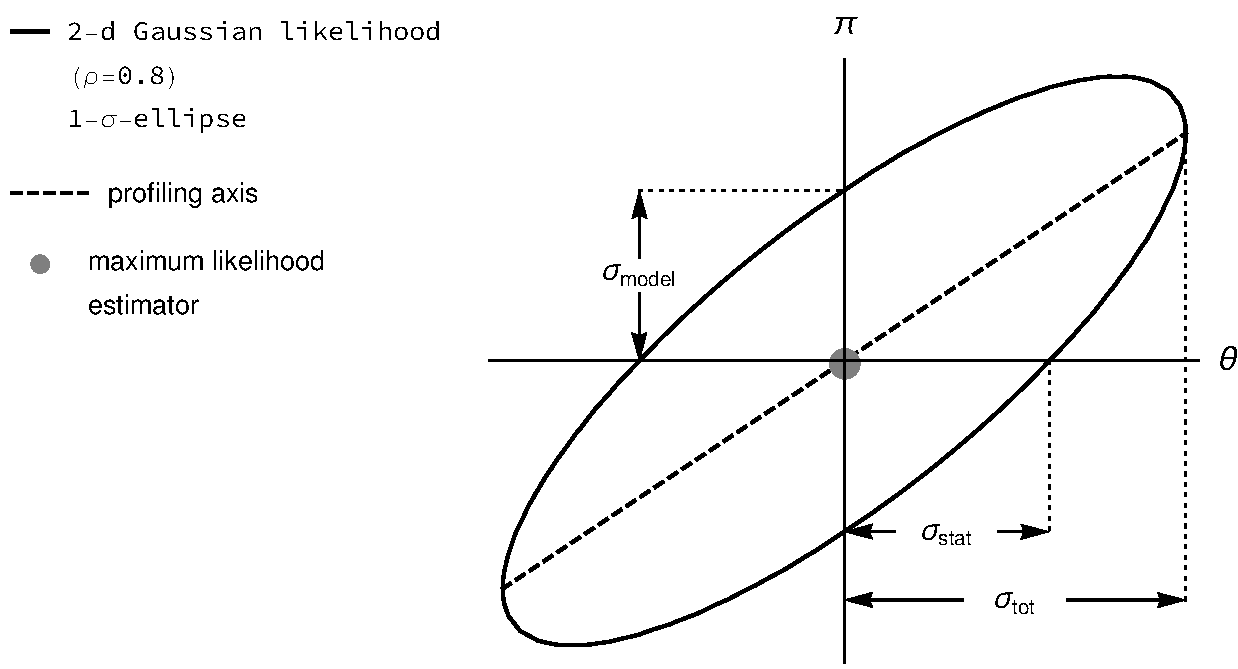
\includegraphics[width=\textwidth]{\currentFigureFolder/profileLikelihood.pdf}
	\xcaption{Illustration of the profile-likelihood method}{Illustration of the profile-likelihood method.}{The graph illustrates the extraction of a confidence interval from the likelihood in a two-dimensional scenario, where there is only one nuisance parameter~$\pi$ and one parameter of interest~$\theta$. The graph is a contour plot of an exemplary two-dimensional likelihood of Gaussian shape with a correlation between $\pi$ and $\theta$ of $\rho=0.8$. The contour encloses a 1-$\sigma$-confidence region as per equation~\eqref{eq:statMethodsConfidenceContour}. Its width in the dimension of~$\pi$ is indicated as ``model''-uncertainty with reference to an uncertainty stemming from a model established by a calibration measurement as described in section~\ref{sec:katrinElossStatisticsCombMeasurements}. The width in the dimension of~$\theta$ stems from the intrinsic statistical uncertainty. The dashed line contains the points~$(\theta, \hat{\hat{\pi}}(\theta))$ as per equation~\eqref{eq:katrinElossStatisticsProfileLikelihoodRatio}. It intersects the contour at the point furthest left and right in the dimension of $\theta$ independently of $\rho$, $\sigma_\mathrm{stat}$ and $\sigma_\mathrm{model}$. The point of intersection determines $\sigma_\mathrm{tot}$. For example, MINOS of the ROOT software framework is an algorithm that numerically tries to find the intersection of the dashed line and the contour~\cite{James1998}. Under the conditions stated in the main text, the interval of width $2\cdot\sigma_\mathrm{tot}$ on the $\theta$ axis around the maximum likelihood estimator is per construction a confidence \mbox{interval (\SI{68}{\percent} C.L.)} for the true value of $\theta$. A feature that can intuitively be deduced from the graph is the following: No matter how much $\sigma_\mathrm{model}$ is reduced, the total uncertainty $\sigma_\mathrm{tot}$ can never shrink below $\sigma_\mathrm{stat}$. Likewise, whether a longer measurement, that decreases $\sigma_\mathrm{stat}$, can improve $\sigma_\mathrm{tot}$ depends on $\sigma_\mathrm{model}$ and the correlation $\rho$.}
	\label{fig:katrinElossStatisticsProfileLikelihood}
\end{figure}
Apart from the parameters of interest $\paramVec$, the KATRIN likelihood can depend on further nuisance parameters $\nuisanceParamVec$. With regard to the study presented in this chapter, the parameter of interest is the squared neutrino mass $\paramVec\equiv\nuMass^2$ and the nuisance parameters are the further three parameters of a nominal four-parameter KATRIN neutrino mass fit as well as the parameters of the energy loss model (KATRIN or Aseev). The derivation of a combined confidence region for the full parameter set may cause long run times (or be impossible) due to the dimensionality (here: 15 parameters of the KATRIN model and additional four parameters of a nominal KATRIN neutrino mass fit). And, more importantly, as indicated by the naming conventions, only a confidence interval for the squared neutrino mass is of interest. The aim of KATRIN is the deduction of a stand-alone confidence interval for the neutrino mass as opposed to an interval that depends on many other nuisance parameters. This section outlines the profile-likelihood method, that effectively handles nuisance parameters in the derivation of a one-dimensional confidence interval.

\paragraph{Confidence Regions for the Parameters Of Interest Only}
Section~\ref{sec:statMethodsUncertaintyIntervalsConfidence} already introduced a method for deriving confidence regions for the full parameter set that the likelihood depends on (parameters of interest and nuisance parameters) based on the likelihood ratio as a test statistic. It can be used to reject estimators for the combined parameter set with a significance of $\alpha$ and include all non-rejected estimators in a confidence region of confidence level $\alpha$. The same approach may also be used to construct a confidence region only for the parameters of interest. But, in the strict frequentist approach, values for the parameters of interest $\paramVec$ are excluded from the confidence region only if they are rejected for all possible values of the nuisance parameters~\cite{ReviewOfParticlePhysics}. To show the rejection for all possible values of the nuisance parameters may be difficult~\cite{ReviewOfParticlePhysics} (corresponding studies were not pursued in the scope of this thesis). The difficulty may be circumvented if a test statistic is found that solely depends on the parameters of interest. Exact independence from the nuisance parameters is only achievable in special cases, it can, however, be achieved approximately by the use of the profile-likelihood ratio as test statistic~\cite{ReviewOfParticlePhysics}.

\paragraph{The Profile-Likelihood Ratio}
In the following, the profile likelihood is defined. It only depends on the parameters of interest $\paramVec$ and is independent of the nuisance parameters $\nuisanceParamVec$. Its values correspond to the likelihood values evaluated at $\paramVec$ in the dimensions of the parameters of interest and maximized in the dimensions of the nuisance parameters~\cite{ReviewOfParticlePhysics}
\begin{equation}
\label{eq:katrinElossStatisticsProfileLikelihood}
\profLikelihood(\paramVec) = 
L(\paramVec, \hat{\hat{\nuisanceParamVec}}(\paramVec))
\comma
\end{equation}
where the double-hat indicates the maximization respectively the ``profiling''. Also, the profile-likelihood ratio can be defined~\cite{ReviewOfParticlePhysics}
\begin{equation}
\label{eq:katrinElossStatisticsProfileLikelihoodRatio}
\lambda_\mathrm{p}(\paramVec) = 
\frac{\profLikelihood(\paramVec)}{\profLikelihood(\hat{\paramVec})}
\fullstop
\end{equation}
According to Wilks’ theorem~\cite{wilks1938}, the distribution of $-2\ln\lambda_\mathrm{p}(\hat{\paramVec})$, where $\hat{\paramVec}$ is the \gls{mle} (see section~\ref{sec:statMethodsMLE}), approaches a chi-square distribution in the limit of a large data sample, independently of the values of the nuisance parameters $\nuisanceParamVec$~\cite{ReviewOfParticlePhysics}. Hence, the profile- likelihood ratio offers a test statistic, based on which, values for the parameters of interest can be rejected. In other words, the profile-likelihood method is a constructive approach on how to derive a confidence interval for the parameters of interest. 

Figure~\ref{fig:katrinElossStatisticsProfileLikelihood} illustrates the profile-likelihood method for the case where $\paramVec$ and $\nuisanceParamVec$ are one-dimensional. It also illustrates how the inclusion of nuisance parameters in order to avoid systematic shifts (for example in order to account for the uncertainties of the parameters of the KATRIN energy loss model) widens the likelihood and enlarges the uncertainties of the parameters of interest.

\subsection{An Asimov Data Set in Relation to Ensemble Tests in Sensitivity Studies}
\label{sec:katrinElossStatisticsAsimov}
If one were to repeat the KATRIN experiment many times, one would obtain an ensemble of confidence intervals for the neutrino mass (see section~\ref{sec:statMethodsUncertaintyIntervalsConfidence} about confidence intervals and also see table~\ref{tab:statMethodsSensitivityFromEnsembleTests} with sensitivity studies from former works where the statistical portion of the sensitivity is listed with an uncertainty, which implies a distribution of statistical uncertainties). KATRIN's sensitivity can be deduced from a confidence interval (see section~\ref{sec:statMethodsSensitivtyDef} about KATRIN's sensitivity). In that sense, if many KATRIN measurements are simulated, one also obtains an ensemble respectively a distribution of sensitivities. One way to obtain this distribution is to simulate many KATRIN neutrino mass measurements and fluctuate the measured electron counts according to Poissonian statistics (or Gaussian statistics as an approximation). The expectation value for KATRIN's sensitivity can than be extracted from the obtained distribution. The simulation of many measurements was for example applied within the scope of the KATRIN Design Report~\cite{Angrik:2005ep}. It should be noted, that a distribution of sensitivities is narrow compared to its expectation value (see for example table~\ref{tab:statMethodsSensitivityFromEnsembleTests} where the spread of the statistical uncertainty on the squared neutrino mass is smaller than the mean value by three orders of magnitude).

Instead of simulating many experiments, the median of KATRIN's sensitivity might be obtained from one simulation. Simulating a KATRIN neutrino mass measurement can be time-consuming depending on its level of detail. In that regard, using only one simulation is more practical. The median for KATRIN's sensitivity might be retrieved from one simulation by replacing the electron count rates with their expectation value instead of fluctuating them according to Poissonian statistics~\cite{Cowan2011}. This reasoning is based on Walt's theorem~\cite{Wald1944} that concerns the sum of Gaussian distributed random variables in the limit of many summands (which approximately conforms the KATRIN-chi-square likelihood). Such a single simulated data set is called an Asimov\footnote{The name of the Asimov data set is inspired by the short story ``Franchise'', by Isaac Asimov. In the story, elections are held by selecting the single most representative voter to replace the entire electorate~\cite{Cowan2011}.} data set. However, whether this approach is applicable may be hard to verify without doing an ensemble test, which would nullify the practicality here.

In the scope of this chapter, both approaches, using an Asimov data set and simulating an ensemble, were applied. The outcome verifies that an Asimov data set would be representative in the study presented in this chapter and indeed yields the median sensitivity.